%--------------------------------------------------------------------------------------------------
\chapter{Aufbau des Konzepts}\label{cha:AufbauDesKonzepts}

In diesem Kapitel wird der Aufbau des Konzepts erklärt. Daher gibt es zu erst einen Einblick in den Digitalisierungsprozess von Produktionseinlagen. Daraufhin wird diese Arbeit in das Gesamtkonzept der Mensch-Maschine Interaktion eingeordnet. Schließlich wird der Aufbau des Modells mithilfe des Functional-Mockup Interfaces erklärt.

%--------------------------------------------------------------------------------------------------
\section{Von der physischen Produktionsanlage zum virtuellen Klon}\label{sec:PhysischZumKlon}

Um die Produktionsabläufe einer Fabrik in einer virtuellen Welt abzubilden gibt es insgesamt sieben Schritte die befolgt werden müssen.

\begin{enumerate}
	\item \textbf{Scannen der Fabrik} \\
	Im ersten Schritt werden die Produktionsräume inklusive der Produktionsanlagen gescannt. Das Ergebnis dieses Scans ist eine Punktwolke.
	\item \textbf{Umwandlung des Scans} \\
	Der Scan muss von einer Punktewolke in CAD Modelle umgewandelt werden. Da die CAD Modelle zu groß und daher unpraktikabel für die Entwicklungsumgebung Unity sind, werden diese in das OBJ Format umgewandelt. Die Modelle sind für den späteren Aufbau des virtuellen Klons der echten Produktionsanlage notwendig.
	\item \textbf{Abbildung: Produktionsanlage $\rightarrow$ Modell} \\
	Es wird ein physisches Modell zur Darstellung einiger wichtiger Herausforderungen der echten Produktionsanlage gebaut. Dies könnte Beispielsweise die Form einer Produktionsstraße mit mehreren Stationen besitzen.
	\item \textbf{Virtueller Aufbau} \\
	Das physische Modell der echten Produktionsanlage aus Schritt drei wird in der virtuellen Welt abgebildet (virtueller Klon) und mit dem Menschmodell begehbar gemacht. Dieser Schritt erlaubt die virtuelle Planung einer Produktionsanlage.
	\item \textbf{Konnektivität und Kommunikation} \\
	Die Produktionsanlagen des physischen Modells werden mit der Cloud vernetzt um eine bidirektionale Kommunikation zwischen dem physischem Modell und dem virtuellen Klon zu ermöglichen.
	\item \textbf{Interaktion} \\
	Die Interaktion mit zwischen dem Bediener und den Produktionsanlagen in der virtuellen Welt wird implementiert. Es müssen unter Umständen anwendungsspezifische Benutzeroberflächen implementiert werden.
	\item \textbf{Skalierung} \\
	Skalierung der Vorgehensweise durch Anwendung von Schritt vier bis sechs auf die echte Produktionsanlage.
\end{enumerate}
Durch das Einhalten dieser Schritte erhält man einen virtuellen Klon der echten Produktionsanlage. Diesen virtuellen Klon kann man für viele Zwecke einsetzen, dazu gehören Beispielsweise die Produktionsplanung oder das Fernsteuern von Produktionsanlagen. Das Ergebnis dieser Arbeit kommt bei Schritt vier und sechs zum Einsatz [Quelle Yübo?].

%--------------------------------------------------------------------------------------------------
\section{Mensch-Maschine Interaktion im Kontext dieser Arbeit}\label{sec:MMInteraktion}
\begin{figure}[h]
	\centering
	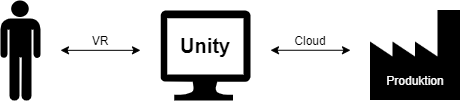
\includegraphics[width=0.7\linewidth]{Bilder/A19_MMI}
	\caption{Mensch-Maschine Interaktion im Kontext dieser Arbeit, eigene Abbildung}
	\label{fig:MMI}
\end{figure}
\noindent Durch die Abbildung der echten Produktionsanlage in der virtuellen Welt findet die Mensch-Maschine-Interaktion in zwei Schritten statt. Im ersten Schritt interagiert der Mensch mit der Software (dem Computer) über VR-Hardware. Dieser Computer interagiert dann über eine Cloud mit der echten Produktionsanlage. Die Kommunikation findet in beiden Schritten bidirektional statt.
\newline\newline
Diese Arbeit befasst sich mit dem ersten Schritt der oben erklärten Mensch-Maschine Interaktion. Für dem Rest dieser Arbeit werden wir annehmen, dass es bereits eine geeignete Infrastruktur für die Kommunikation zwischen dem Computer und der Produktionsanlage über eine Cloud gibt.

%--------------------------------------------------------------------------------------------------
\section{Das Modell der Interaktivität mit einem Menschmodell}\label{sec:ModellAufbau}
Basierend auf den im folgenden definierten Anforderungen soll mit Hilfe des Functional-Mockup Interfaces ein Modell aufgebaut werden.

\subsection{Anforderungen an das Modell}\label{sec:AnforderungenKonzept}
Da das Modell aus zwei Teilen besteht, haben beide Teile Ihre eigenen Anforderungen. Diese werden im Folgenden erläutert. Das Ziel ist es ein Menschmodell zu schaffen, welches interaktiv mit seiner Umgebung interagieren kann.

\subsubsection{Menschmodell}\label{sec:AnforderungenMensch}
\begin{enumerate}
	\item \textbf{Genauigkeit} \\
	Die Genauigkeit der Abbildung der Tracking-Daten auf das virtuelle menschliche Abbild ist von zentraler Bedeutung. Vor allem in einem Szenario, bei dem sich mehrere virtuelle menschliche Abbildungen in einem virtuellen Klon einer Produktionsanlage aufhalten ist die möglichst genaue Abbildung unabdingbar, um Beispielsweise auf andere Bediener in der virtuellen Welt Rücksicht nehmen zu können.
	\item \textbf{Echtzeit} \\
	Sowohl das Tracking des Bedieners als auch die Abbildung der Tracking-Daten auf das virtuelle menschliche Abbild sind echtzeitkritische Anwendungen. Die Verzögerungen müssen möglichst gering sein um eine gute Nutzbarkeit zu ermöglichen.
	\item \textbf{Interoperabilität} \\
	Das Menschmodell muss umgebungsunabhängig implementiert werden. Dies bedeutet, dass das Menschmodell in beliebigen Umgebungen (Fabriken, Produktionshallen, etc.) eingesetzt werden kann.
	\item \textbf{Modularität} \\
	Sowohl einzelne Komponenten als auch das ganze Menschmodell an sich unterliegen der Anforderung der Modularität, um in Zukunft Verbesserungen oder Erweiterungen am Modell durchführen zu können.
\end{enumerate}

\subsubsection{Interaktion}\label{sec:AnforderungenInteraktion}
\begin{enumerate}
	\item \textbf{Bidirektionalität} \\
	Der Informationsaustausch muss bidirektional stattfinden. Das bedeutet, dass der Bediener über geeignete, leicht zu verstehende, optisch ansprechende und vor allem einheitliche Benutzeroberflächen interagieren kann. Einerseits ermöglichen diese Benutzeroberflächen dem Bediener das Interagieren mit Produktionsanlagen, andererseits werden auf diesen Benutzeroberflächen für den Bediener relevante Informationen in geeigneter Form dargestellt.
	\item \textbf{Genauigkeit} \\
	Auch bei der Interaktion spielt die Genauigkeit eine wichtige Rolle. Der Bediener sollte intuitiv, mit relativ geringen Lernaufwand, schnell und vor allem präzise mit der Umgebung interagieren können.
	\item \textbf{Echtzeit} \\
	Die Interaktion muss mit einer möglichst geringen Verzögerung stattfinden, um dem Nutzer schnelle Reaktionen und spontane Anpassungen oder Verbesserungen zu ermöglichen.
	\item \textbf{Interoperabilität} \\
	Die Interaktion muss über eine einheitliche Schnittstelle stattfinden um Interoperabilität zu gewährleisten, sodass sich die Funktionalität auf beliebige Maschinen und Produktionsanlagen übertragen lässt.
	\item \textbf{Modularität} \\
	Durch das Gewährleisten der Modularität wird sichergestellt, dass die Interaktion in Zukunft auch auf neue VR-Hardware übertragen werden kann ohne das die gesamte Software neu geschrieben werden muss.
\end{enumerate}
Durch das Einhalten dieser Herausforderungen ergibt sich ein Menschmodell, welches in Echtzeit die Bewegungen des Bedieners auf das virtuelle Menschliche Abbild projiziert. Des Weiteren ermöglicht das Modell dem Bediener in der virtuellen Welt mit dem virtuellen Klon der Produktionsanlage zu interagieren. Da von Anfang an ein Fokus auf Interoperabilität und Modularität gelegt wird, ist das ganze Modell erweiterbar und an verschiedene Hardware und unterschiedliche Einsatzzwecke anpassbar.

\subsection{Das Functional-Mockup Interface}\label{sec:DasFMU}
Das Functional-Mockup Interface (FMI) ist ein ursprünglich von der Daimler AG entwickelter unabhängiger Standard für den Austausch von dynamischen Modellen und Co-Simulation. Zum Einsatz kommt das Functional-Mockup Interface beispielsweise beim Modellaustausch oder der Co-Simulation zwischen Zulieferern und den OEMs (Original Equipment Manufacturer) [24, FMI-Paper, S.1].
Anfang 2010 wurde die erste Version (Version 1.0) des FMI Standards veröffentlicht, welche zunächst nur den Modellaustausch unterstützte. Einige Monate später folgte dann die Unterstützung für Co-Simulation. Mittlerweile gab weitere Nachfolger Versionen. Die aktuellste Version (Version 2.0.1) wurde im Oktober 2019 veröffentlicht, unterscheidet sich aber von der Vorgängerversion (Version 2.0) aus dem Jahr 2014 nur durch einige Bugfixes [2, FMI-Spez, S.2].
Da es neben den anwendungsspezifischen Standards (z.B. Matlab/Simulink: S-Functions) zunächst keinen unabhängigen Standard für den Austausch von Modellen oder die Co-Simulation gab [24, FMI-Paper, S.1], liegt der größte Vorteil des FMI-Standards in seiner Unabhängigkeit.
\newline
Wie bereits erwähnt gibt es für den FMI Standard zwei übergeordnete Anwendungsszenarien:
\begin{enumerate}
	\item \textbf{Modellaustausch} \\
	Der FMI Standard ermöglicht Modellierungsumgebungen ein dynamisches System Modell in C-Code zu repräsentieren, sodass dieses Modell auch in anderen Modellierungsumgebungen genutzt werden kann. Ermöglicht wird dies durch die Darstellung der Modelle mit Hilfe von mathematischen Gleichungen (z.B. Algebraische Gleichungen, Differentialgleichungen oder Diskrete Gleichungen), welche auch Zeit-, Zustands- oder Schritt-Events enthalten können. Es werden große Modelle und sowohl die offline als auch die online Simulation unterstützt [25, FMI-Spez, S.4].
	\item \textbf{Co-Simulation} \\
	Des Weiteren ermöglicht der FMI Standard das Verbinden von mehreren Subsystem, welche über vordefinierte Kommunikationsschnittstellen kommunizieren und somit eine Co-Simulationsumgebung schaffen. Dabei wird der Datenaustausch und die Synchronisation zwischen den einzelnen Subsystemen durch einen sogenannten Master Algorithmus gesteuert. Bei den Master Algorithmen ist zu beachten, dass diese kein Teil des eigentlichen FMI Standards sind [25, FMI-Spez, S.4]. Daher sind die Master Algorithmen nicht standardisiert und können unterschiedliche zusätzliche Funktionalitäten wie z.B. den Austausch von Variablen unterstützen [24, FMI-Paper, S.1].
\end{enumerate}
Die grundlegenden Komponenten die beim Einsatz des FMI Standards immer zum Einsatz kommen sind das „FMI Application Programming Interface (C)“ und das „FMI Description Schema (XML)“. Ersteres enthält dabei alle benötigten Gleichungen des Models. Dabei kommt die Programmiersprache C zum Einsatz, da sie portabel ist und auch für den Einsatz in eingebetteten System geeignet ist. Die XML-Datei (vgl. Abbildung \ref{fig:FMIOverview}) hingegen enthält die Definitionen aller Variablen in einem standardisierten Format. Diese Variablendefinition ist durchaus eine komplexe Datenstruktur. Die Simulationstools können selber entscheiden wie sie mit diesen Daten umgehen und wie sie die Daten in ihren Programmen repräsentieren möchten. Dieser Ansatz erlaubt das Speichern und Laden der Variablendefinitionen ohne Einbußen bei der Performance in der Programmiersprache der Simulationsumgebung, wie z.B. C\# oder Java [25, FMI-Spez, S8].
\begin{figure}[h]
	\centering
	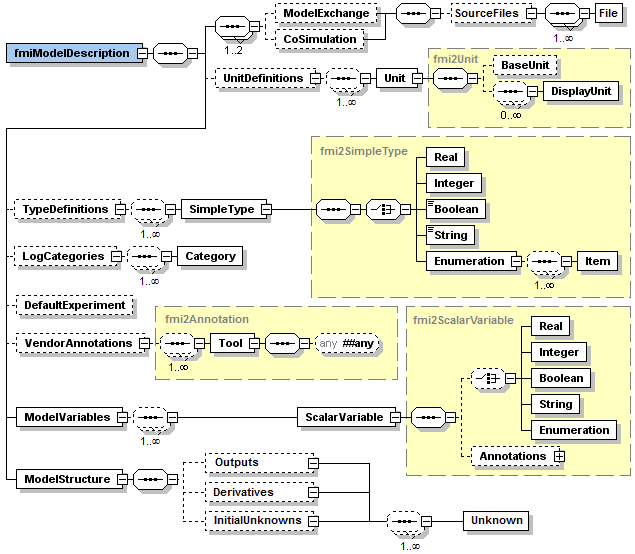
\includegraphics[width=0.7\linewidth]{Bilder/A20_FMIOverview}
	\caption{Aufbau der FMI Variablenbeschreibung [25, FMI-Spez, S.30]}
	\label{fig:FMIOverview}
\end{figure}
\newline
Da das FMI nur ein Interface ist wird eine Instanz des Interfaces FMU (Functional-Mockup Unit) genannt. Das FMI Interface soll den Einsatz von FMUs in beliebigen Simulationsumgebungen einfach gestalten. Dafür werden durch die Simulationsumgebung Funktionen des FMI aufgerufen um ein FMU zu generieren. Es ist zusätzlich anzumerken, dass eine FMU beliebig oft und sogar als Teil von anderen Modellen generiert werden kann [25, FMI-Spez., S.8]. Eine FMU wird in einer ZIP-Datei mit der Endung „.fmu“ bereitgestellt und kann neben den bereits angesprochenen Komponenten (C-Code und XML-Datei) zusätzliche Anwendungsspezifische Daten wie Icons oder Dokumentationen enthalten [25, FMI-Spez, S.4+9] In Abbildung \ref{fig:FMIBlock} ist eine Instanz einer FMU illustriert. Eine FMU enthält neben den Eingabeparametern (Rot) und den Ausgabeparametern (Blau) noch interne Werte. Zu den internen Werten gehört die Zeit t, interne Parameter p und nach außen sichtbare Variablen v [25, FMI-Spez, S.8].
\begin{figure}[h]
	\centering
	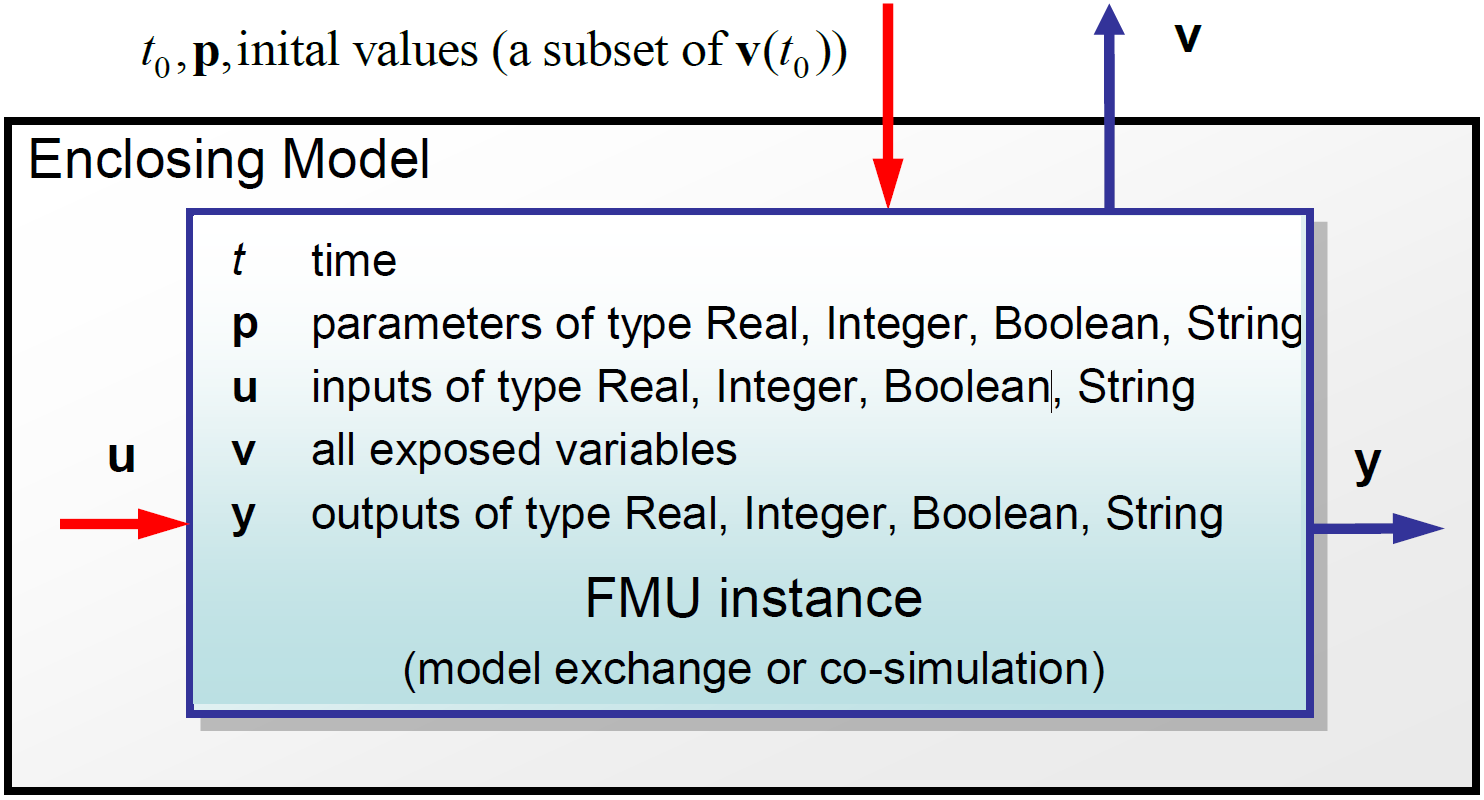
\includegraphics[width=0.5\linewidth]{Bilder/A21_FMIBlock}
	\caption{FMU Instanz [25, FMI-Spez, S.9]}
	\label{fig:FMIBlock}
\end{figure}
\newline
In der Abbildung \ref{fig:FMUEinordnung} ist noch einmal dargestellt, wie das Zusammenspiel zwischen der Simulationsumgebung, der FMU und dem FMI aussieht. Die Simulationsumgebung liest Variablendefinition (XML) der FMU, welche dem FMI Standard entspricht. Dies ermöglicht der Simulationsumgebung eine oder mehrere Instanzen der FMU zu generieren. Aufgrund dieser Struktur kann jede Simulationsumgebung eine eigene Benutzeroberfläche einsetzen und selber entscheiden wie die Daten repräsentiert werden.
\begin{figure}[h]
	\centering
	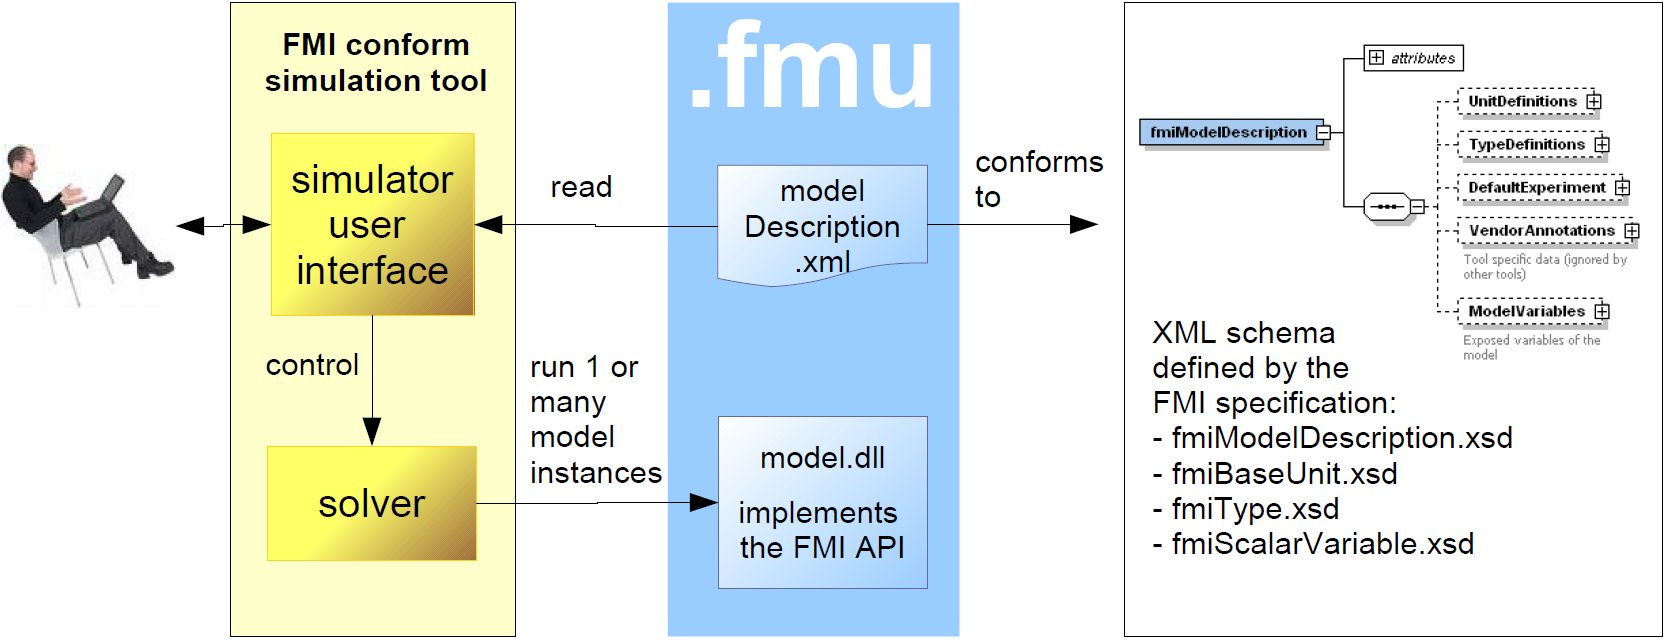
\includegraphics[width=1\linewidth]{Bilder/A22_User-FMU-FMI}
	\caption{Funktionsweise der FMU in der Simulationsumgebung [26, QTronic, S.7]}
	\label{fig:FMUEinordnung}
\end{figure}

\subsection{Der Aufbau des Models}\label{sec:ModelAufbau}
Um die in Kapitel \ref*{sec:AnforderungenKonzept} erläuterten Herausforderungen umzusetzen soll mit Hilfe des in Kapitel \ref*{sec:DasFMU} eingeführten FMI Standards ein theoretisches Modell geschaffen werden, wie ein Menschenmodell mit der Möglichkeit mit der Umgebung zu interagieren aufgebaut sein könnte. Daher wird im Folgenden vorgestellt, wie die Variablendefinition im XML-Format und das eigentliche Modell in C-Code auszusehen hätten.

\subsubsection{Variablendefinition (XML)}\label{sec:Variablendefinition}
Wie in Abbildung \ref{fig:FMIOverview} dargestellt besteht die XML-Datei aus mehreren Komponenten. Nicht alle Komponenten sind für jeden Einsatzzweck relevant, daher werden im Folgenden die relevanten Komponenten genauer erläutert.

\paragraph{Attributes}\label{sec:AttributeFMU}
\noindent Neben den in Abbildung \ref{fig:FMIOverview} dargestellten Elementen, enthält die XML-Datei noch das Element „Attributes“. Es gibt insgesamt 12 mögliche Attribute, jedoch sind nur vier zwingend notwendig [25, FMI-Spez, S.33].
\begin{enumerate}
	\item \textbf{fmiVersion} \\
	Dieses Attribut gibt an, welche Version des FMI Standards bei der Generierung der XML-Datei
	eingesetz wurde [25, FMI-Spez, S.33].
	\item \textbf{modelName} \\
	Durch dieses Attribut wird dem Modell ein Name zugewiesen [25, FMI-Spez, S.33].
	\item \textbf{guid} \\
	Durch das Attribut „guid“ (Globally Unique Identifier) wird sichergestellt, dass die XML-Datei 
	Kompatibel ist mit den C-Funktionen der FMU. Dafür wird in der Regel eine Art Fingerabdruck
	generiert und in den C-Funktionen hinterlegt [25, FMI-Spez, S.33].
	\item \textbf{variableNamingConvention} \\
	Dieses Attribut bestimmt ob die Namen der variablen einer bestimmten Konvention 
	unterliegen. Standardmäßig wird hier der Token „flat“ verwendet, wenn alle Variablen
	in einer Liste von Strings vorliegen [25, FMI-Spez, S.33].
	\item \textbf{description (optional)} \\
	In diesem Attribut kann auf Wunsch eine kurze Beschreibung der FMU hinterlegt werden [25, 
	FMI-Spez, S.33].
	\item \textbf{author (optional)} \\
	Dieses Attribut ermöglicht es Angaben über die Autoren (Entwickler) zu machen [25, FMI-
	Spez, S.33].
	\item \textbf{version (optional)} \\
	Um einen besseren Überblick über die verschiedenen Versionen einer FMU zu ermöglichen,
	kann in diesem Attribut die Versionsnummer (z.B. Version 1.0) hinterlegt werden [25, FMI-
	Spez, S.33].
	\item \textbf{copyright (optinal)} \\
	In diesem Attribut können Informationen über das Copyright hinterlegt werden [25, FMI-
	Spez, S.33].
	\item \textbf{license (optional)} \\
	Es besteht die Möglichkeit durch dieses Attribut angaben über die Lizenz für die Verwendung
	der FMU zu machen [25, FMI-Spez, S.33].
	\item \textbf{generationTool (optional)} \\
	In diesem Attribut kann der Name des Tools mit dem die XML-Datei generiert wurde
	hinterlegt werden [25, FMI-Spez, S.33].
	\item \textbf{generationDateAndTime (optional)} \\
	Dieses Attribut ermöglicht es das Datum und die genaue Uhrzeit der Generierung der XML-
	Datei zu hinterlegen. Dabei wird das Format „YYYY-MM-DDThh:mm:ssZ“ verwendet. Das
	„T“ soll lediglich das Datum von der Uhrzeit trennen und das „Z“ steht für die Zeitzone
	(Greenwich Meantime) [25, FMI-Spez, S.33].
	\item \textbf{numberOfEventIndicators (optional)} \\
	Falls die FMU für Co-Simulation verwendet wird, wird dieses Attribut ausgelassen. Ansonsten
	wird hier die Anzahl der Indikatoren für Events beim Einsatz der FMU für Modellaustausch
	hinterlegt [25, FMI-Spez, S.33].
\end{enumerate}
Abbildung \ref{fig:FMUAttribute} illustriert, wie die Attribute für die FMU aussehen könnten.
\begin{figure}[h]
	\centering
	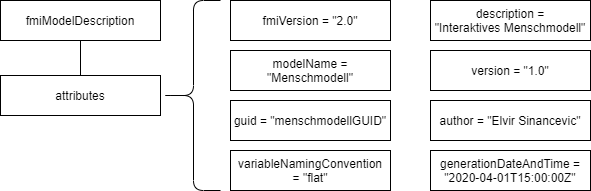
\includegraphics[width=1\linewidth]{Bilder/A24_FMUAttributBeispiel}
	\caption{Darstellung der Attribute für das Menschmodell, eigene Abbildung}
	\label{fig:FMUAttribute}
\end{figure}

\paragraph{ModelExchange / Co-Simulation}\label{sec:ModellExchangeCoSimulation}
\noindent Dieses Element gibt an, ob die FMU für Modellaustausch und/oder Co-Simulation ausgelegt ist.
Falls das Element „ModelExchange“ vorhanden ist, enthält die FMU entweder selbst das eigentliche Modell oder die Kommunikationsschnittstelle zu einem Tool, welches das Modell enthält. Die Simulationsumgebung kümmert sich dann um die Simulation.
Falls jedoch das Element „CoSimulation“ vorhanden ist, enthält die FMU selbst das Modell und kümmert sich selbst um die Simulation, oder enthält die Kommunikationsschnittstelle zu einem Tool welches das Modell enthält und sich selbst um die Simulation kümmert. Die Simulationsumgebung enthält den in Kapitel \ref*{sec:DasFMU} bereit angesprochenen Master Algorithmus, um mehrere FMUs gemeinsam in einer Co-Simulationsumgebung einzusetzen  [25, FMI-Spez, S.30].
Es ist noch wichtig anzumerken, dass mindestens eins der beiden Elemente vorhanden sein muss, um den Typ der FMU zu definieren [25, FMI-Spez, S.31].
Da das Menschmodell sowohl das Modell enthält als auch die Simulation (hier: Abbildung der Bewegungsdaten auf das virtuelle menschliche Abbild) eigenständig übernimmt, müsste die FMU auf Co-Simulation ausgelegt werden [25, FMI-Spez, S.30].
\newline
In Abbildung \ref{fig:FMUCoSimulation} ist illustriert, wie die FMU als Teil einer Anwendung funktionieren würde.
\begin{figure}[h]
	\centering
	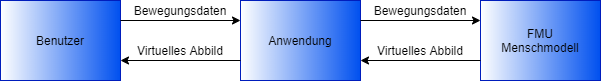
\includegraphics[width=1\linewidth]{Bilder/A23_FMUCoSimulation}
	\caption{Funktionsweise der FMU als Teil einer Anwendung, eigene Abbildung}
	\label{fig:FMUCoSimulation}
\end{figure}

\paragraph{UnitDefinitions}\label{sec:1}
\noindent bla bla blabla bla blabla bla blabla bla blabla bla blabla bla blabla bla blabla bla 

\paragraph{TypeDefinitions}\label{sec:2}
\noindent bla bla blabla bla blabla bla blabla bla blabla bla blabla bla blabla bla blabla bla 

\paragraph{LogCategories}\label{sec:3}
\noindent bla bla blabla bla blabla bla blabla bla blabla bla blabla bla blabla bla blabla bla 

\paragraph{DefaultExperiment}\label{sec:4}
\noindent bla bla blabla bla blabla bla blabla bla blabla bla blabla bla blabla bla blabla bla 

\paragraph{VendorAnnotations}\label{sec:5}
\noindent bla bla blabla bla blabla bla blabla bla blabla bla blabla bla blabla bla blabla bla 

\paragraph{ModelVariables}\label{sec:6}
\noindent bla bla blabla bla blabla bla blabla bla blabla bla blabla bla blabla bla blabla bla 

\paragraph{ModelStructure}\label{sec:7}

\subsubsection{Grober Aufbau des Codes}\label{sec:CCode}
In der Abbildung \ref{fig:CCodeDarstellung} ist ein stark vereinfachter Überblick über den Aufbau des Codes dargestellt. Die VR Hardware ist über das Programm VIVE Wireless mit der VR-Schnittstelle für Computer SteamVR verbunden. In dem Projekt ist zusätzlich das SteamVR Plugin für die Entwicklungsumgebung Unity installiert, welches die Schnittstelle zwischen dem Projekt und der VR-Hardware vollendet. Zur Verfügung gestellt wird das Modell von dem Plugin „Final IK“ (IK = Inverse Kinematics), welches gleichzeitig die Kalibrierung, die Berechnung der inversen Kinematik und die Abbildung der Bewegungsdaten auf das Modell übernimmt. Die wichtigsten Klassen sind die Klassen „Calibration Controller“ und „TrackerAssignment“. Die Klasse „Calibration Controller“ ruft zunächst die Methode für die Zuweisung der Tracker in der Klasse „TrackerAssignment“ auf, bevor der Kalibrierungsprozess gestartet wird. Durch die Klasse „Tracker Assignment“ werden nur die aktiven Tracker den entsprechenden Körperteilen (Füße, Knie, Steißbein, Hände, Ellenbogen, Kopf) zugewiesen. Die getrackten Körperteile enthalten das Skript „SteamVR Tracked Object“, über welches sie die Bewegungsdaten des Bedieners erhalten. Es ist anzumerken, dass das Menschenmodell noch über weitere Funktionalitäten, wie z.B. die Interaktion mit der Umgebung verfügt. Einen genaueren Einblick in den Aufbau des Projektes gibt es in Kapitel XX.
\begin{figure}[h]
	\centering
	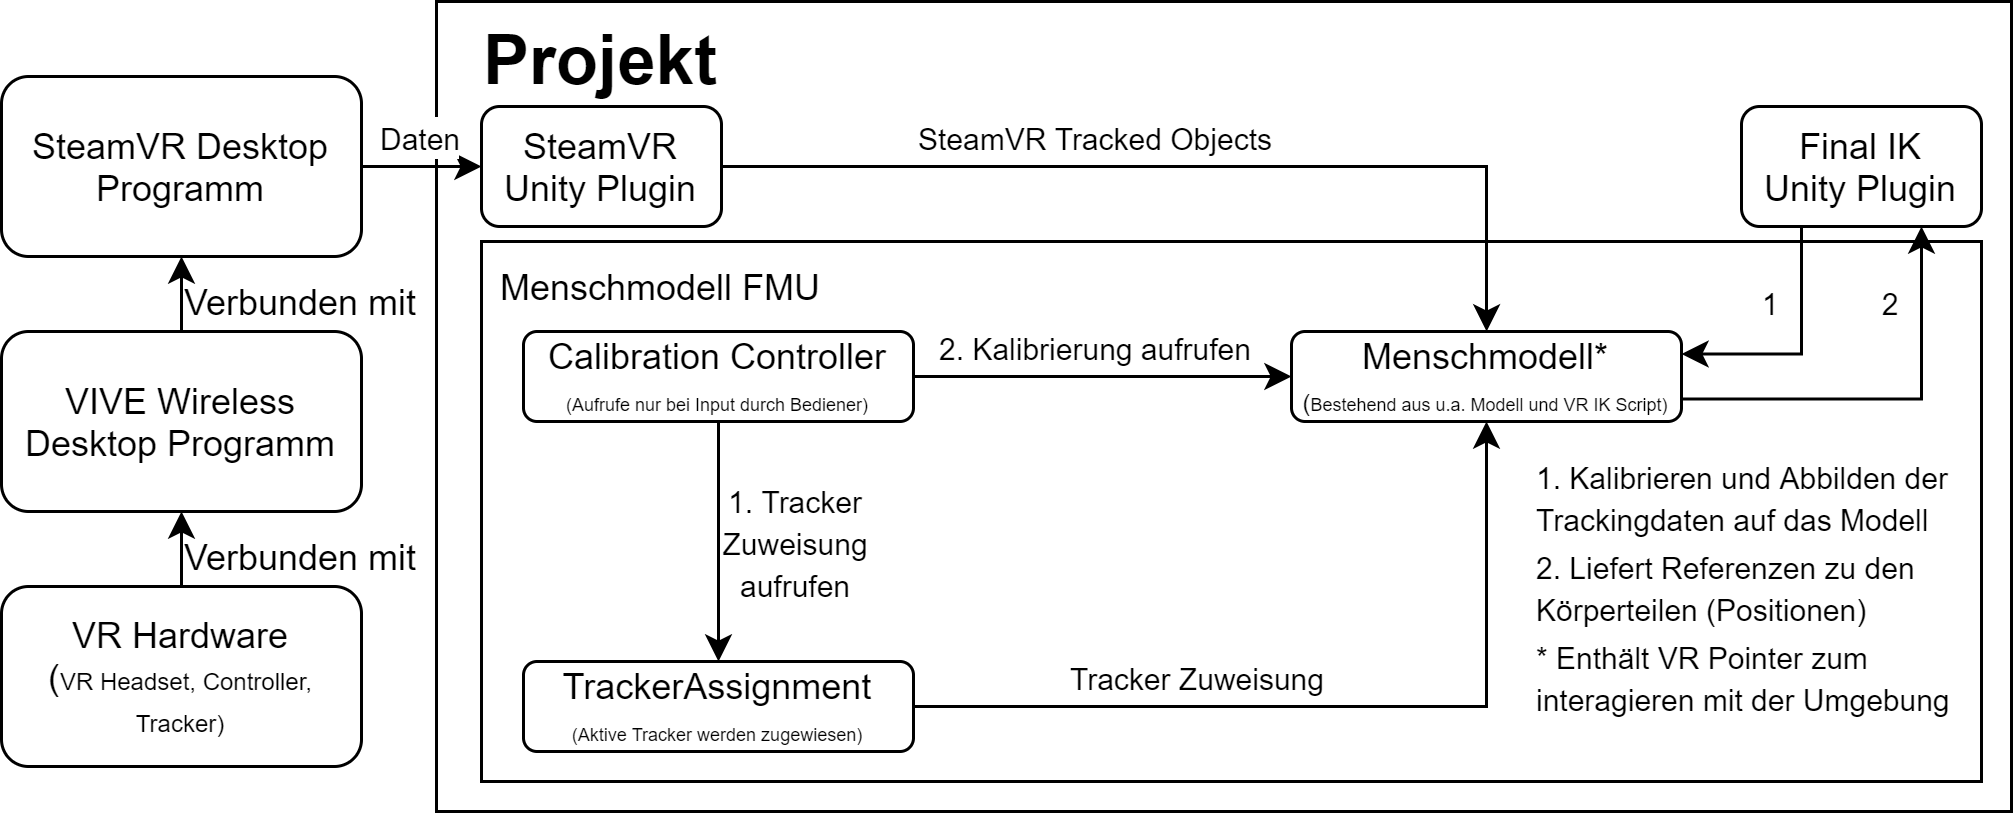
\includegraphics[width=1\linewidth]{Bilder/A25_CCodeDarstellung}
	\caption{Aufbau des Codes (grobe Darstellung), eigene Abbildung}
	\label{fig:CCodeDarstellung}
\end{figure}

\subsection{Potenziale}\label{sec:PotenzialeFMU}
bla bla blabla bla blabla bla blabla bla blabla bla blabla bla blabla bla blabla bla blabla bla blabla bla blabla bla blabla bla blabla bla blabla bla blabla bla blabla bla blabla bla blabla bla bla
%--------------------------------------------------------------------------------------------------